\section{Durchführung}
\label{sec:Durchführung}

Der Versuch besteht aus zwei Teilen, die im Folgenden getrennt beschreiben werden.
\subsection{Erster Teil}
In diesem Teil des Versuchs wird die Dampfdruckkurve von Wasser zwischen 30 bis 1000 $mbar$ bestimmt.
\begin{figure}
    \centering
    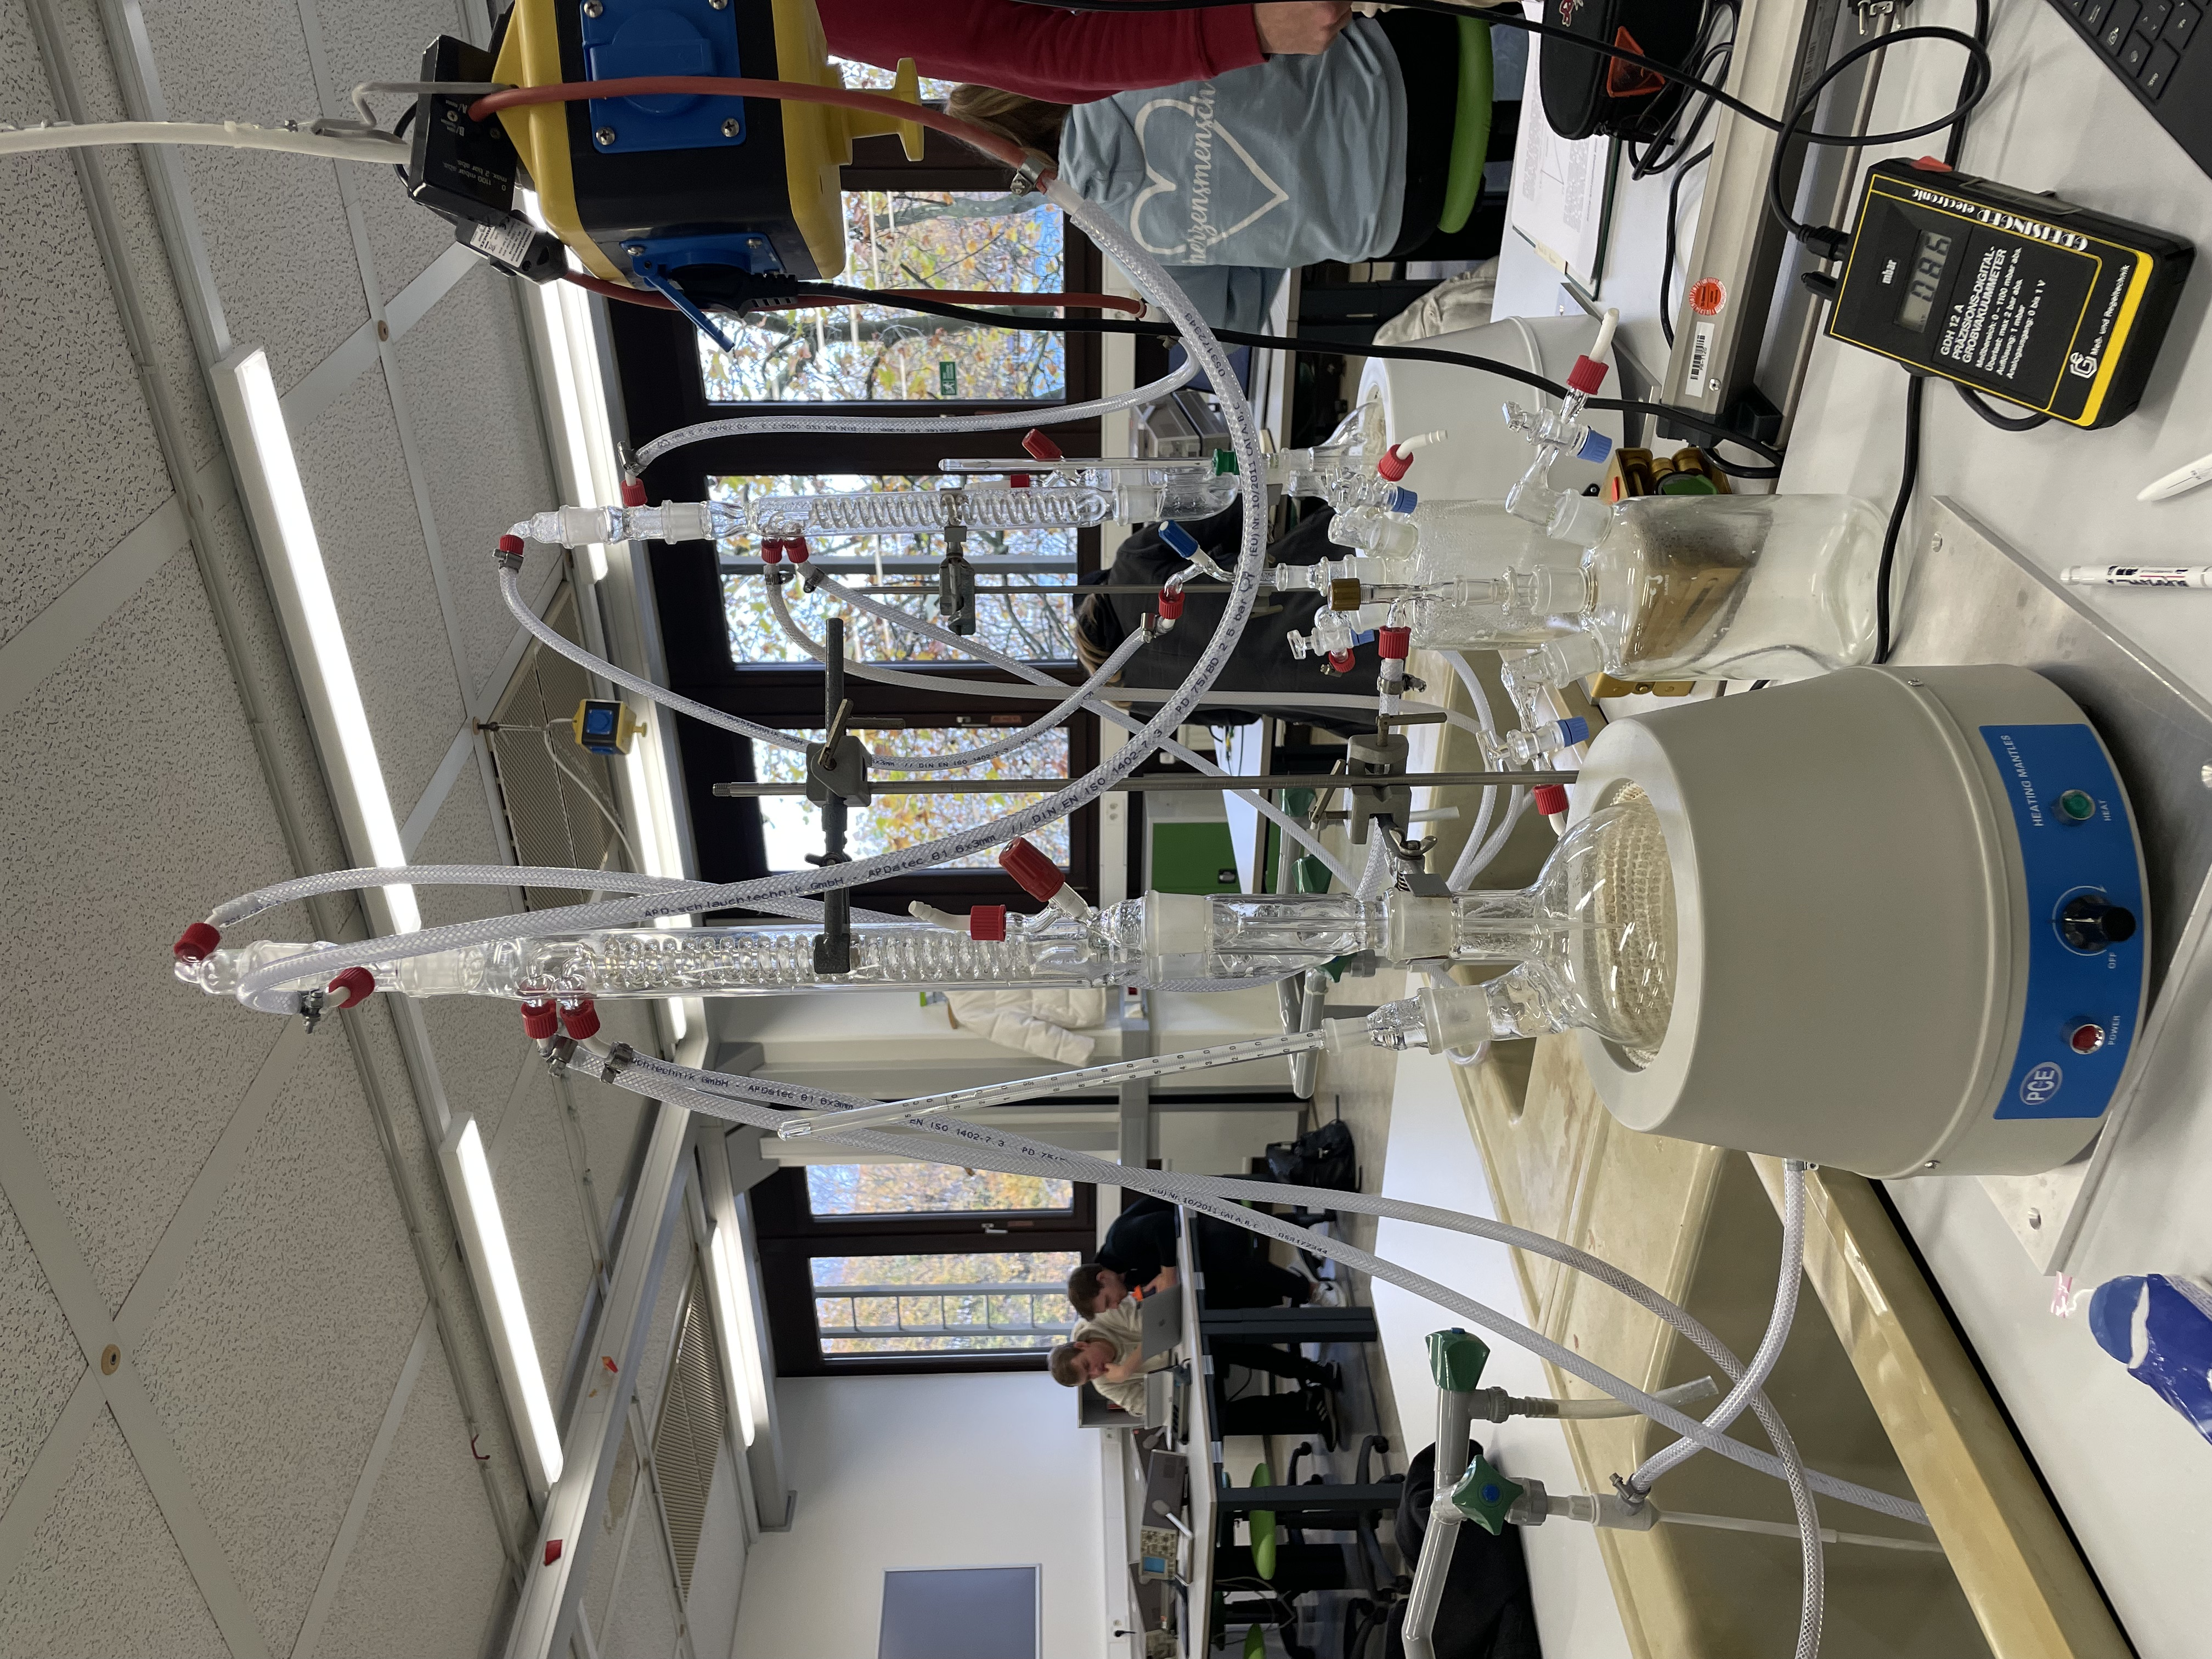
\includegraphics[height=3cm, angle=270]{content/Verwendete_Messapparatur.jpeg}
    \caption{Zu sehen ist die verwendete Messapparatur während der Evakuierung.}
    \label{Abb:Messapparatur}
\end{figure}
Eine Wasserstrahlpumpe ist über die Woulffsche Flasche mit dem Rest der Apparatur verbunden.
Diese Flasche lässt sich durch ein Absperrhahn und ein Drosselventiel abriegeln, was im Verlauf des Versuchs noch wichtig ist.
\begin{figure}
    \centering
    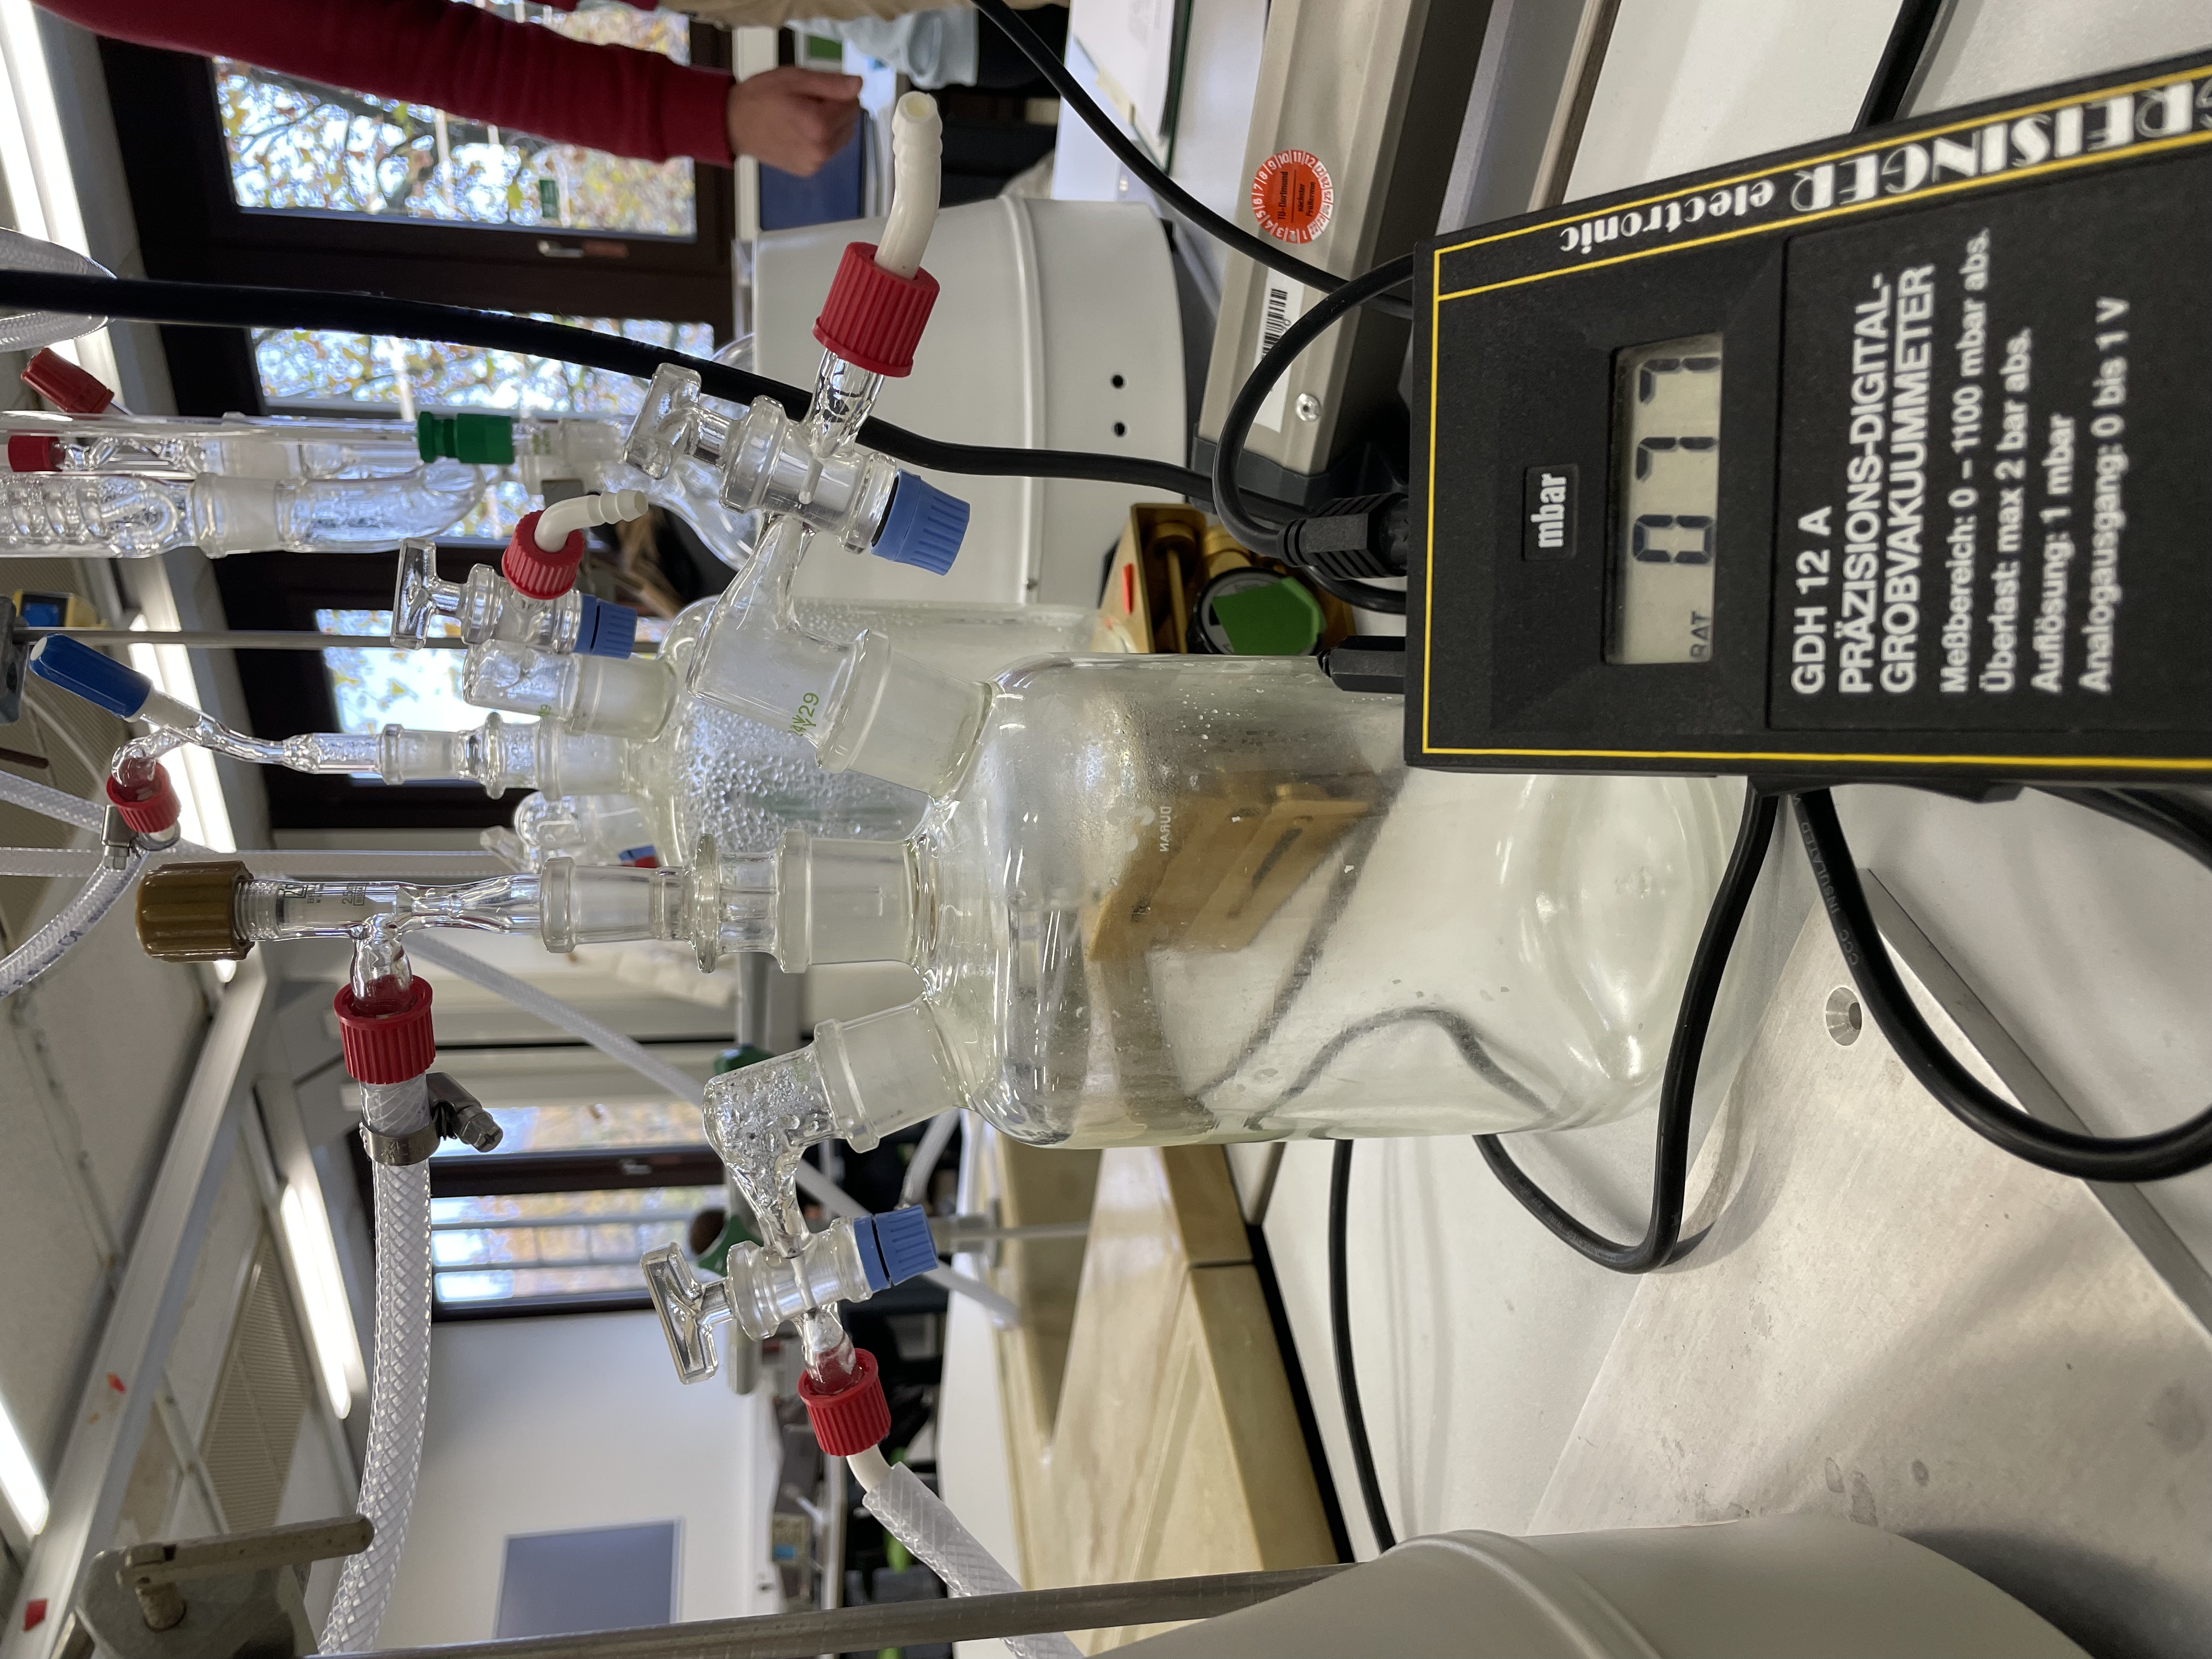
\includegraphics[height=3cm, angle=270]{content/Woulffsche_Flasche.jpeg}
    \caption{Ein Foto der Woulffsche Flasche und des Manometers während der Evakuierung der Apparatur.}
    \label{Abb:Woulffsche_Flasche}
\end{figure}
Ein Manometer ist ebenfalls mit der gesamten Apparatur verbunden, um kontinuierlich den Druck im Inneren messen zu können.
Nun folgt die eigentliche Apparatur.
Sie besteht aus einer Heizhaube, die einen Mehrhalskolben erhitzt.
In diesem Kolben befindet sich die zu untersuchende Flüssigkeit.
In diesem Fall handelt es sich um Wasser.
Außerdem befindet sich im Kolben ein Thermometer, so kann die Temperatur zu jeder Zeit abgelesen werden.
Ein Rückflusskühler macht die Messapparatur komplett.
Er lässt die aufsteigenden Dämpfe kondensieren, damit sich nicht in das Manometer gelangen.

Zunächst wird die ganze Apparatur mittels der Wasserstrahlpumpe evakuiert, bis der Druck auf 30 $mbar$ abgesunken ist.
Anschließend wird das Drosselventiel geschlossen.
Dann wird der Absperrhahn verschlossen.
So wird die Apparatur nicht weiter evakuiert und die Messung kann beginnen.

Hierfür wird die Heizhaube angeschaltet und der Druck in Abhängigkeit der Zeit gemessen bis der maximale Messwert des Mometers errreicht ist.
Für dieses Manometer war der Wert bei 1100 $mbar$.

\subsection{Zweiter Teil}
Im zweiten Teil des Versuchs wird eine ähnliche Messung für den Druckbereich von 1 bis 15 $mbar$ durchgeführt.
Hierfür muss jedoch eine andere Messapparatur verwendet werden, da die Obige diesem Druck nicht mehr standhalten würde.

Bei dieser Apparatur besteht aus einem Stahlbolzen, der in der Mitte durchgebohrt wurde.
Der Stahlbolzen befindet sich über einer Heizapparatur.
In dem Hohlraum befindet sich die Flüssigkeit, in diesem Versuch Wasser.
Die Temperatur dieser Flüssigkeit wird über ein Termometer angegeben, welches ins Innere des Stahlbolzen ragt.
Der Druck im Stahlbolzen wird über einen Drucksensor, welcher mit dem Hohlraum verbunden ist, angegeben.

Zu Beginn des Versuchs wird die Heizapparatur angeschaltet.
Dann wird mit steigendem Druck die Temperatur gemessen.